\chapter{Sistema de carregamento}

\section{Lista de materiais}

\begin{table}[H]
\centering
\begin{tabular}{|m{1.8cm} |m{8.8cm}|m{3.5cm}|}
\hline
\begin{center}Quantidade\end{center} & \begin{center}Componente\end{center} &\begin{center} Part Number\end{center} \\\hline

 01&Cabo de Força (1,5m) lec 320 C13 - Fêmea Flexível Tripolar 3x0,75$mm^2$ & lec 320 C13 \\\hline
 
01 &  Tomada de força lec 320 C14 - Macho
& lec 320 C14 \\\hline
  
01& Chave seletora de tensão HH 127/220V  & Chave HH \\\hline
   
01& Transformador 110/220V para 30V 1A & Transformador \\\hline

01&Cabo PP 2x2.5$mm^2$ (1m) & Cabo PP \\\hline

02&Plug Conector Jack J4  Macho & Jack Macho \\\hline

01& Conector Jack J4 DC-015 Fêmea 2.1$mm^2$ &Jack Fêmea \\\hline

01& Capacitor - 1000uF/50V & - \\\hline

02& Diodos 1N4007V & 1N4007  \\\hline

01& Transistor NPN BC547 & BC547\\\hline

01& Regulador de tensão L7812 & L7812 \\\hline

01& Regulador de tensão LM317 &  LM317 \\\hline

01& Resistor 240R - 1/4W & - \\\hline

01& Resistor 1KR  - 1/4W & - \\\hline

01& Resistor 0.12R - 1/4W & - \\\hline

05 & Terminal Faston Fêmea &   DJ623-A6  \\\hline

01 & Metro - Cabo flexível 2,5 mm² Verde & - \\\hline

\end{tabular}
\caption{Lista de componentes}
\end{table}

\section{Ferramentas}

\par Para a soldagem dos componentes eletrônicos na PCI (Placas de Circuito Impresso), conexões dos fios com os dispositivos e fixação da PCI na case de proteção ou outro local, é necessário o uso das seguintes ferramentas e acessórios:

\begin{itemize}
    \item Ferro de Solda ou Estação de Solda (15W-40W)
    \item Solda Estanho em fio 1mm
    \item Esponja metálica ou esponja convencional para limpeza da ponta de solda
    \item Lupa com suporte e pinça, para apoio e manuseio da PCI
    \item Sugador de solda
    \item Chave de fenda/phillips
    \item Alicate de corte pequeno
    \item Alicate de desencapar ou estilete
    \item Multímetro
\end{itemize}

\begin{center}
ATENÇÃO
\begin{figure}[H]
 \centering
 
\includegraphics[scale = 0.1]{Figuras/atenção.png}
\end{figure}
\end{center}

\par Os ferros de solda aquecem a temperaturas superiores a 400ºC. Usar um suporte para ferro de solda decente é fundamental para não se acidentar e sofrer com queimaduras. Além disso, certifique-se de trabalhar em uma área bem ventilada ou use um extrator de fumaça ou exaustor de fumaça. Os vapores do fluxo são tóxicos. Leia atentamente as instruções deste manual. Ao soldar, utilize Equipamentos de Proteção Individual (EPIs), tais como, óculos de segurança e luvas de segurança. Mantenha todo o cabelo, roupas folgadas e joias protegidos e fora do caminho de suas ferramentas. Se a solda que você estiver usando contiver chumbo, lave as mãos após concluir o trabalho.


\subsection{Boas práticas}
\PAR É de bom grado ter alguns cuidados ao montar e manter em boas condições as placas de circuito impresso-PCI que estão sujeito a vários fatores de risco como:
\begin{itemize}
\item \textbf{Mecânicos:}
\begin{itemize}
\item Vibrações
\item flexões nas PCI 
\item choques mecânicos
\end{itemize}
\end{itemize}

\begin{itemize}
\item \textbf{Ambientais:}
\begin{itemize}
\item Umidade em excesso
\item Contaminantes pelo ar 
\item Excesso de luz solar
\end{itemize}
\end{itemize}

\begin{itemize}
\item \textbf{Eletrostático:}
\begin{itemize}
\item Descargas elétricas produzidas por atrito e contato humano sem devidos cuidados
\end{itemize}
\end{itemize}

\par {\textbf{Alguns cuidados devem ser tomados:}}

\begin{itemize}
\item Evitar tocar em partes metálicas dos componentes e nos conectores e minimizar o manuseio o máximo possível evitando danos mecânicos;
\item É recomendável segurar a placa de forma a não tocar nas suas trilhas preferível que o manuseamento da mesma seja feito de forma que a pessoa segura a placa pelas suas bordas/ laterais;  

\item Nunca flexione a placa ou utilize de muita força ao manuseá-la pode acarretar em rompimento das trilhas,rompimentos de ligações  de encaixe;

\item Não deixe os equipamentos perto de recipientes com água e nem molhe-os.
\end{itemize}

\section{Impressão da PCI do Carregador}

\par Para a confecção da placa de circuito impresso foi gerado o arquivo Gerber de cada placa de circuito impresso, sendo gerado um arquivo em formato ZIP disponível em Arquivos Gerber sendo fabricadas com 2 Layers com a placa contendo uma espessura de $1.6 mm$ e peso de cobre de $1 oz$. Para a visualização dos arquivos Gerber é necessário a utilização de um programa de prototipagem de placas de circuito impresso ou um visualizador desse tipo de arquivo disponível para download no site do programa utilizado para o projeto EasyEda como pode se observado na figura \ref{fig:Gerber}. A placa de circuito impresso que será confeccionada é apresentada na figura \ref{trilha-carregador}.

\par Link download arquivos Gerber: \href {https://drive.google.com/drive/folders/1P1pQGE_zuSLOB5qd8zfESWqLDwtyoRKd?usp=sharing}{aqui}
\par Link download do programa vizualizador: \href{https://sourceforge.net/projects/gerbv/files/}{aqui} 

\begin{figure}[H]
  \centering
  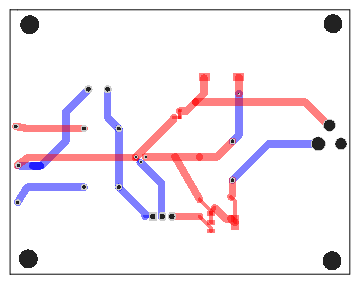
\includegraphics[width=\textwidth]{Figuras/Carregador/PCB_PCB_2020-11-10_21-13-48_2020-11-20_03-04-03.png}
  \caption{Trilhas PCI - Carregador.} 
 %{ \footnotesize Fonte: Autores} 
  \label{trilha-carregador}
\end{figure}

\newpage

\section{Instruções de Montagem do Carregador}

\par A montagem correta da placa é de suma importância para o correto funcionamento do carregador das baterias do projeto, siga os passos a seguir para garantir a correta montagem da placas de circuito impresso e a conexão dos dispositivos da fonte de carregamento.

\begin{figure}[H]
  \centering
  
\includegraphics[scale = 0.15]{Figuras/atenção.png}
\end{figure}


\subsection{PCI do Carregador}
%\subsection{Materiais}
\par Primeiramente é necessário ter em mão todos os componentes para sua montagem \ref{carregador01}.

\begin{figure}[H]
  \centering
  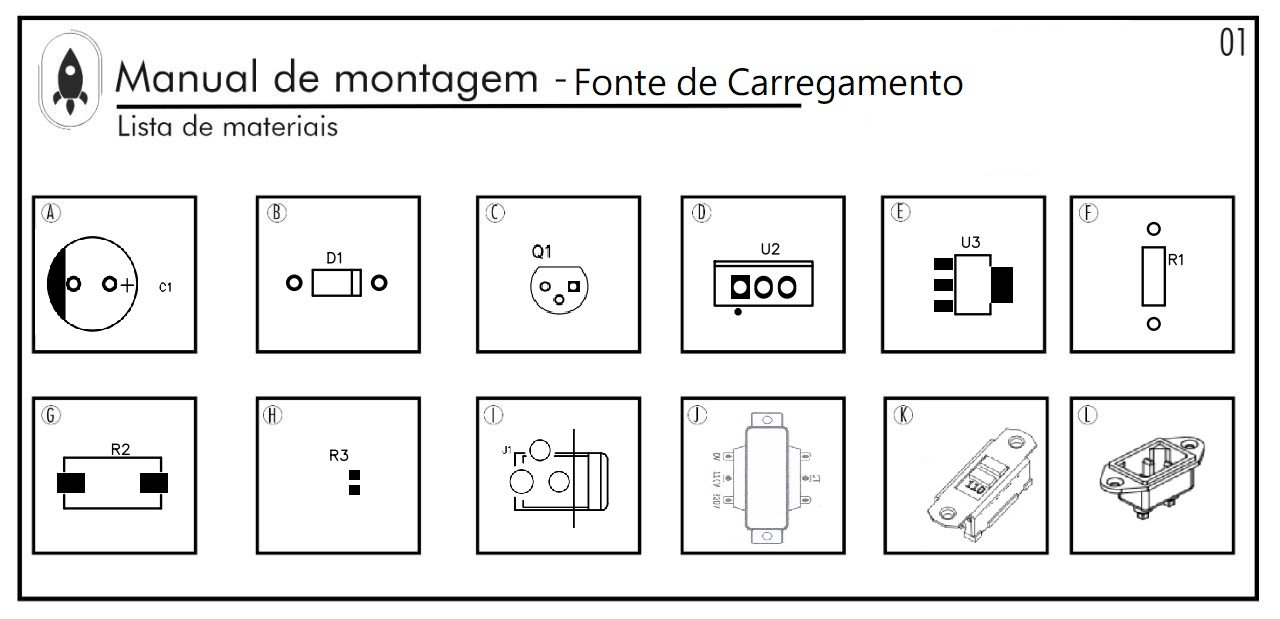
\includegraphics[width=\textwidth]{Figuras/Carregador/carregador_manual_01.jpg}
  \caption{Lista de Materiais - Fonte de Carregamento.} 
 %{ \footnotesize Fonte: Autores} 
  \label{carregador01}
\end{figure}

Com todos os componentes em mãos, pegue componente 'A’(Capacitor - 1000uF/50V), encaixe no local indicado na figura \ref{carregador02} e solde o componente na PCI passando uma fina camada de solda nos terminais e com o uso do alicate cuidadosamente corte as sobras de seus terminais.

\begin{figure}[H]
  \centering
  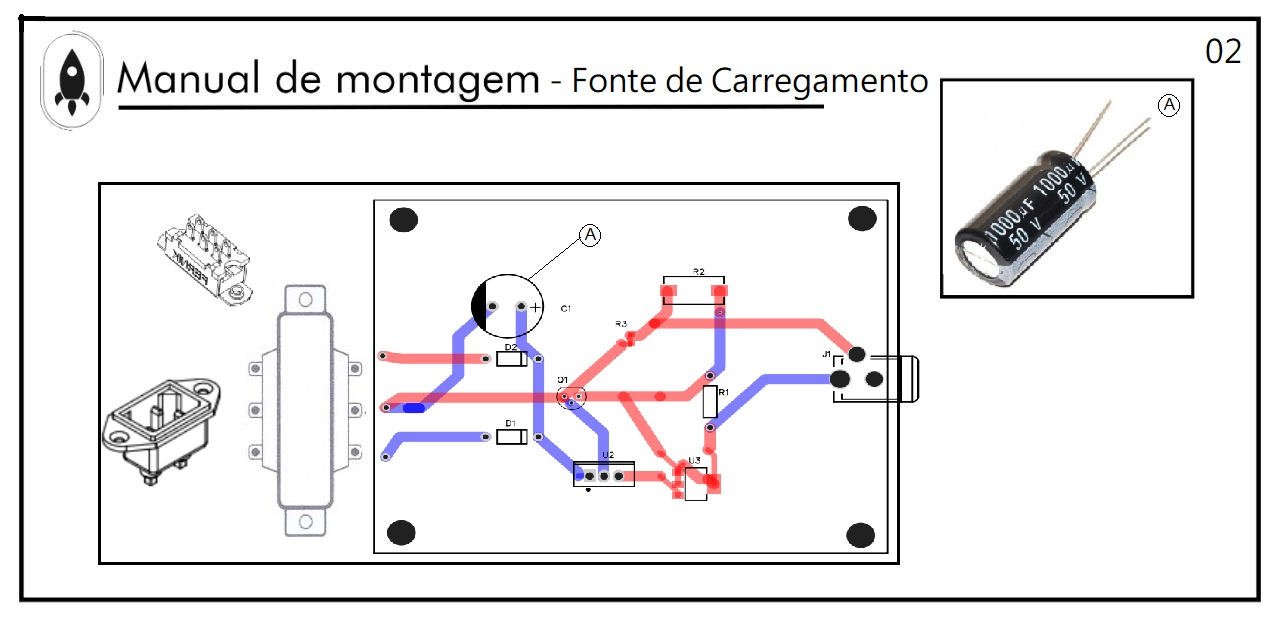
\includegraphics[width=\textwidth]{Figuras/Carregador/carregador_manual_02.jpg}
  \caption{Capacitor - 1000uF/50V.} 
 %{ \footnotesize Fonte: Autores} 
  \label{carregador02}
\end{figure}

Repita o mesmo processo de soldagem para os componentes das figuras \ref{carregador03},  \ref{carregador04}, \ref{carregador05}, \ref{carregador06}, \ref{carregador07}, \ref{carregador08}, \ref{carregador09} e \ref{carregador10}.

\begin{figure}[H]
  \centering
  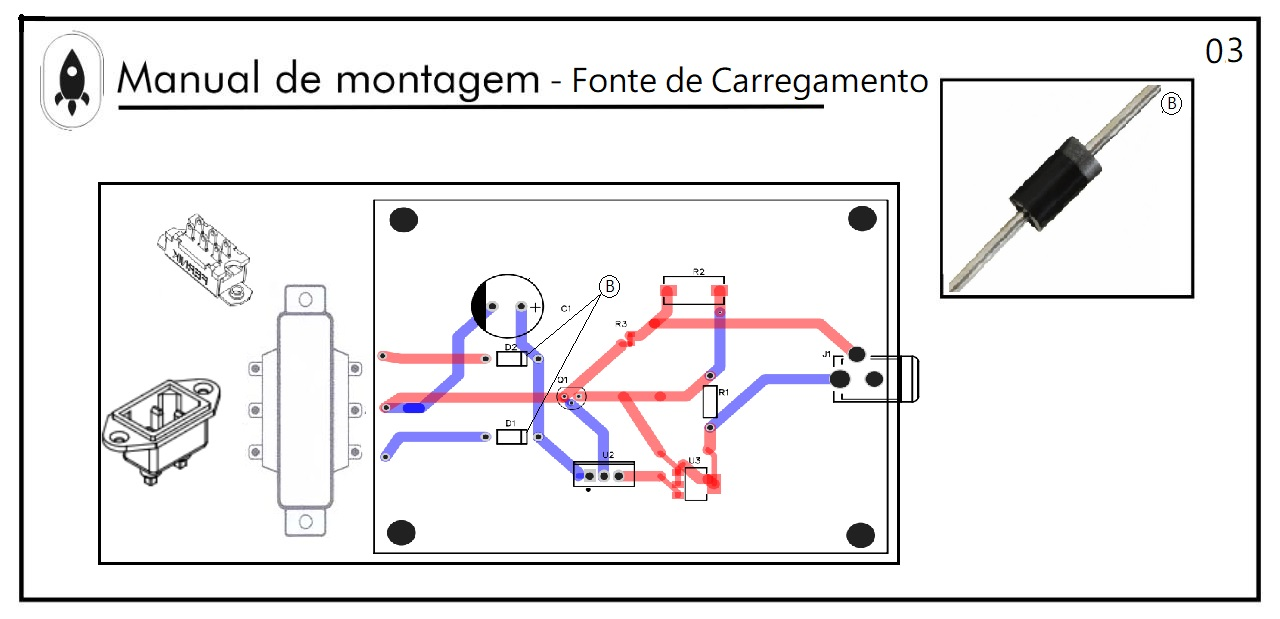
\includegraphics[width=\textwidth]{Figuras/Carregador/carregador_manual_03.jpg}
  \caption{Diodos 1N4007.} 
 %{ \footnotesize Fonte: Autores} 
  \label{carregador03}
\end{figure}

\begin{figure}[H]
  \centering
  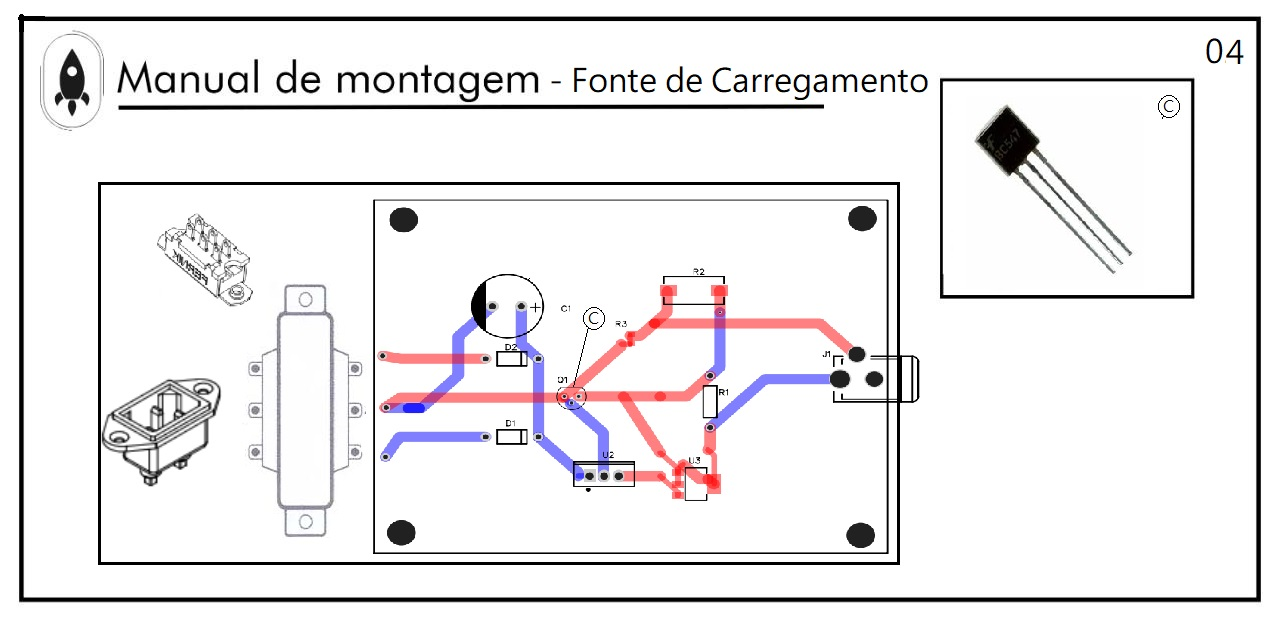
\includegraphics[width=\textwidth]{Figuras/Carregador/carregador_manual_04.jpg}
  \caption{Transistor NPN BC547.} 
 %{ \footnotesize Fonte: Autores} 
  \label{carregador04}
\end{figure}

\begin{figure}[H]
  \centering
  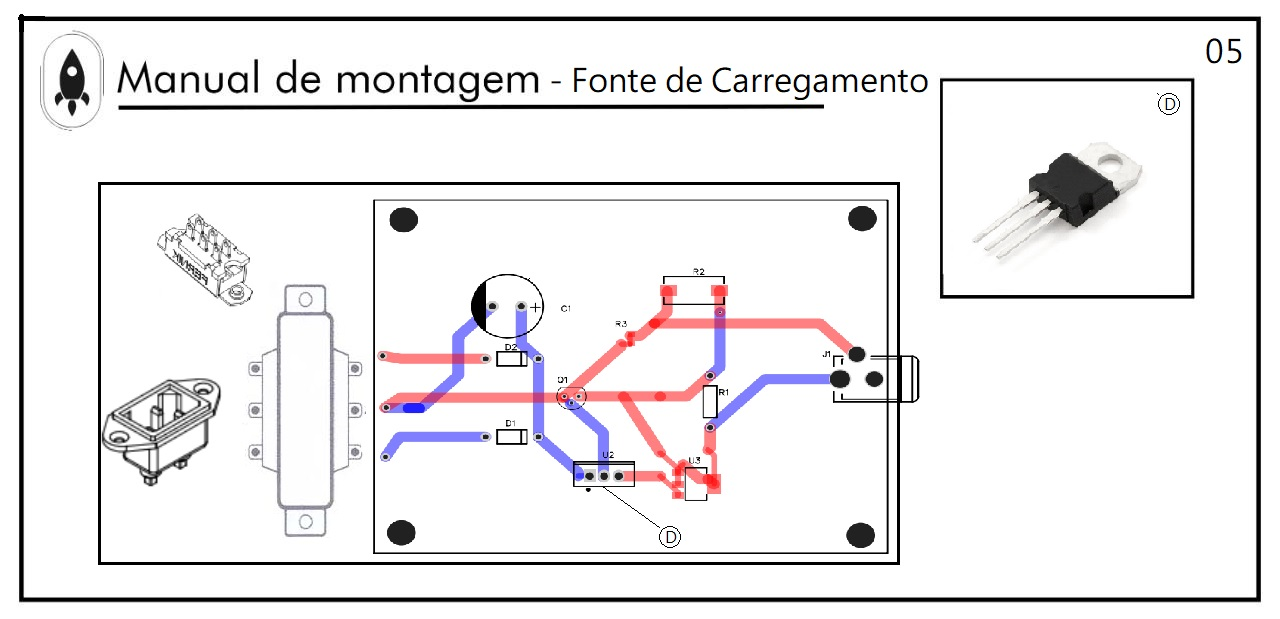
\includegraphics[width=\textwidth]{Figuras/Carregador/carregador_manual_05.jpg}
  \caption{ Regulador de tensão L7812.} 
 %{ \footnotesize Fonte: Autores} 
  \label{carregador05}
\end{figure}

\begin{figure}[H]
  \centering
  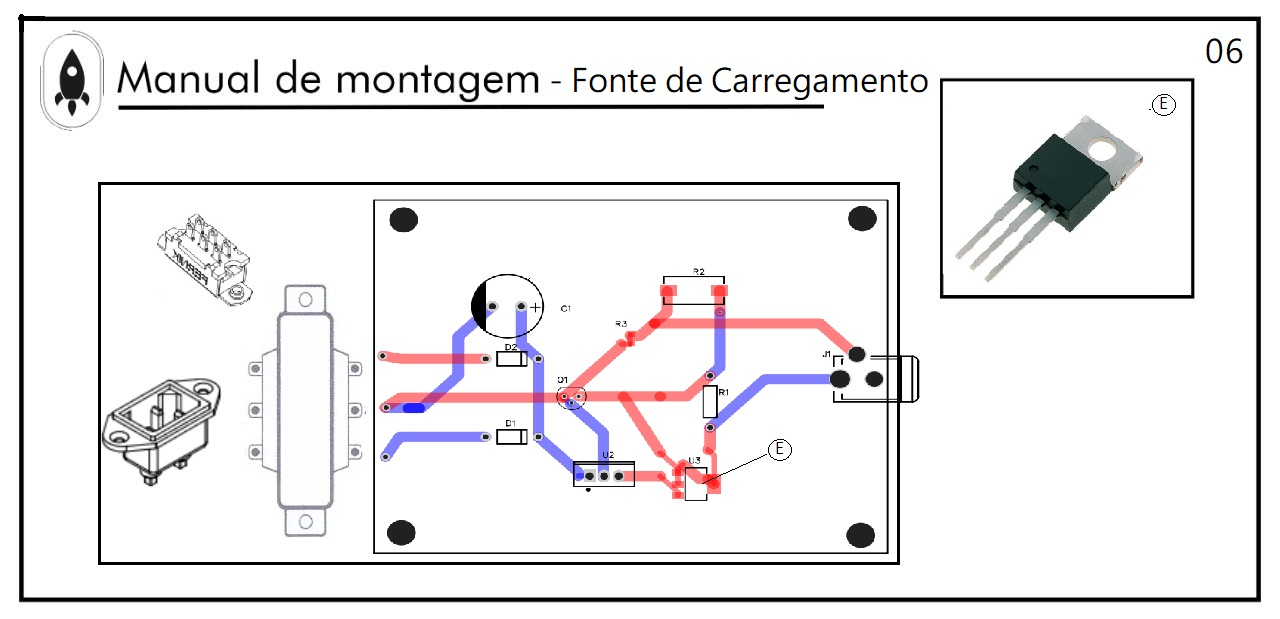
\includegraphics[width=\textwidth]{Figuras/Carregador/carregador_manual_06.jpg}
  \caption{ Regulador de tensão LM317.} 
 %{ \footnotesize Fonte: Autores} 
  \label{carregador06}
\end{figure}

\begin{figure}[H]
  \centering
  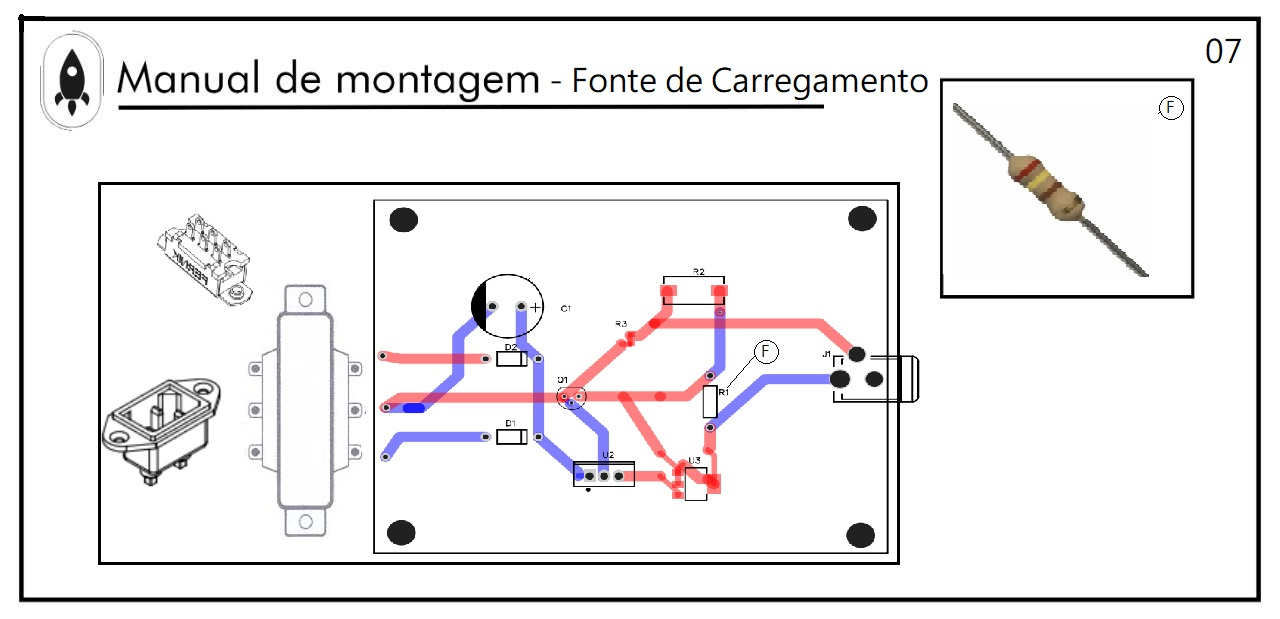
\includegraphics[width=\textwidth]{Figuras/Carregador/carregador_manual_07.jpg}
  \caption{Resistor 240R - 1/4W.} 
 %{ \footnotesize Fonte: Autores} 
  \label{carregador07}
\end{figure}

\begin{figure}[H]
  \centering
  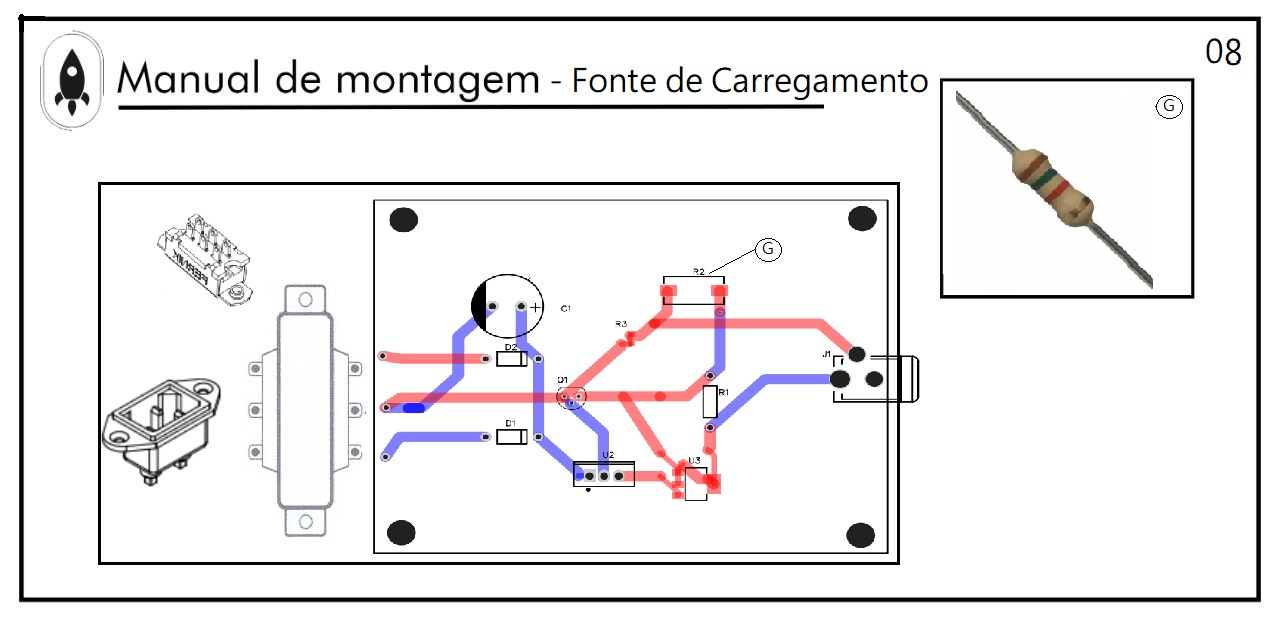
\includegraphics[width=\textwidth]{Figuras/Carregador/carregador_manual_08.jpg}
  \caption{ Resistor 1KR - 1/4W.} 
 %{ \footnotesize Fonte: Autores} 
  \label{carregador08}
\end{figure}

\begin{figure}[H]
  \centering
  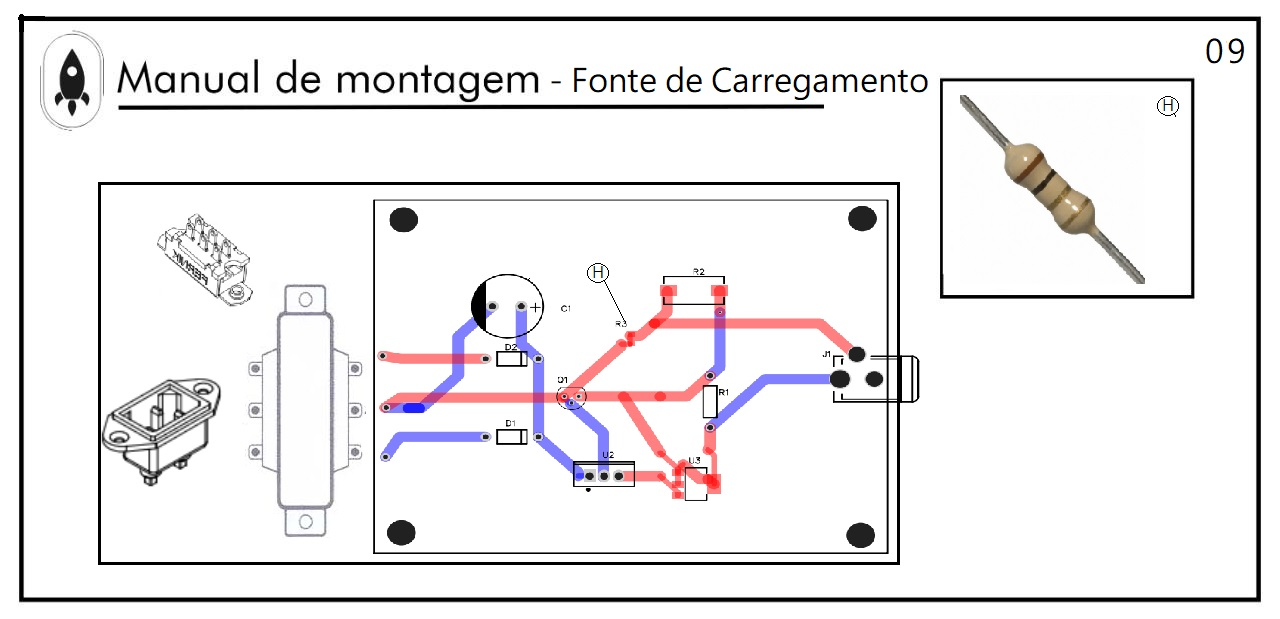
\includegraphics[width=\textwidth]{Figuras/Carregador/carregador_manual_09.jpg}
  \caption{Resistor 0R12 - 1/4W.} 
 %{ \footnotesize Fonte: Autores} 
  \label{carregador09}
\end{figure}

\begin{figure}[H]
  \centering
  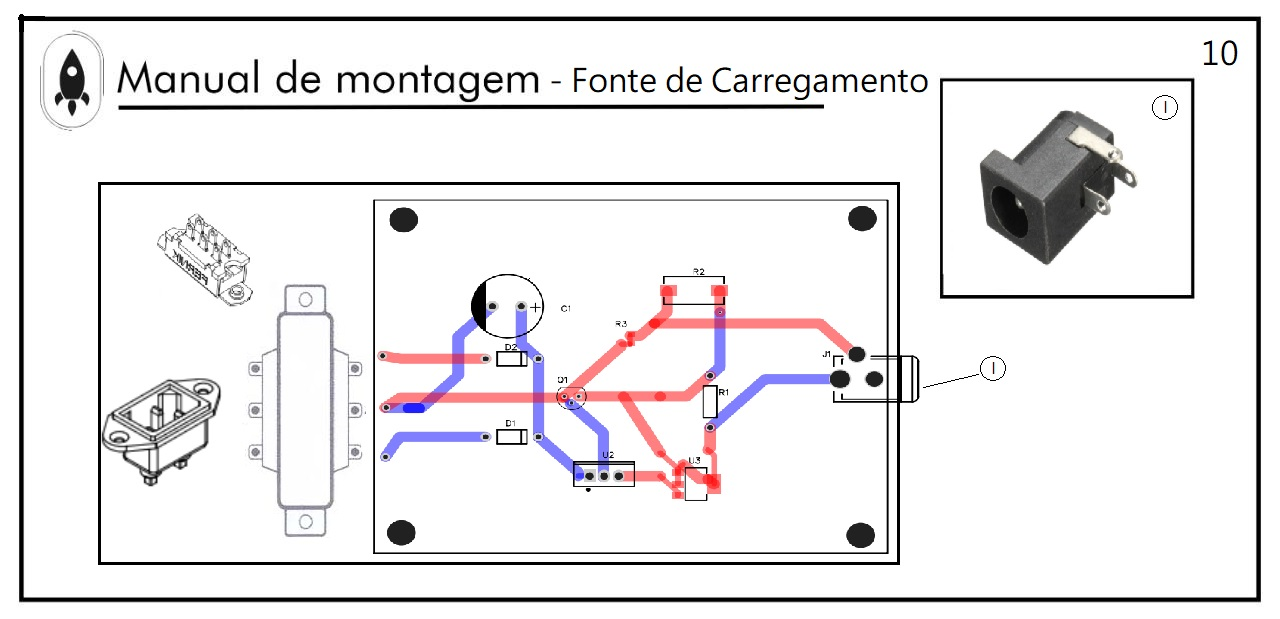
\includegraphics[width=\textwidth]{Figuras/Carregador/carregador_manual_10.jpg}
  \caption{Conector Jack J4 DC Fêmea.} 
 %{ \footnotesize Fonte: Autores} 
  \label{carregador10}
\end{figure}

Depois que todos os dispositivos na PCI estiverem soldados em seus devidos lugares é preciso conectar a placa à estrutura usando uma furadeira e parafusos de 40mm, a parte de fixação será melhor abordada no item 4.4 

Após fixar a PCI na estrutura é preciso fixar o transformador ao seu lado, use o mesmo método de fixação citado anteriormente, para posicionar o transformador corretamente basta posicionar o lado secundário do transformador ao lado da placa PCI de acordo com a figura \ref{carregador11}. Caso no transformador não esteja indicado qual o lado primário e qual o secundário basta seguir os passos a seguir:


\begin{itemize}
    \item Com a ajuda de um multímetro coloque em uma escala baixa de medição de resistência de $200\Omega$ a 1K $\Omega$ 
    \item Com o multímetro meça a resistência entre o fio preto e cada um dos outros dois fios que o acompanha. O lado em que as resistências derem valores maiores esse será o lado primário do transformador.
\end{itemize}


\begin{figure}[H]
  \centering
  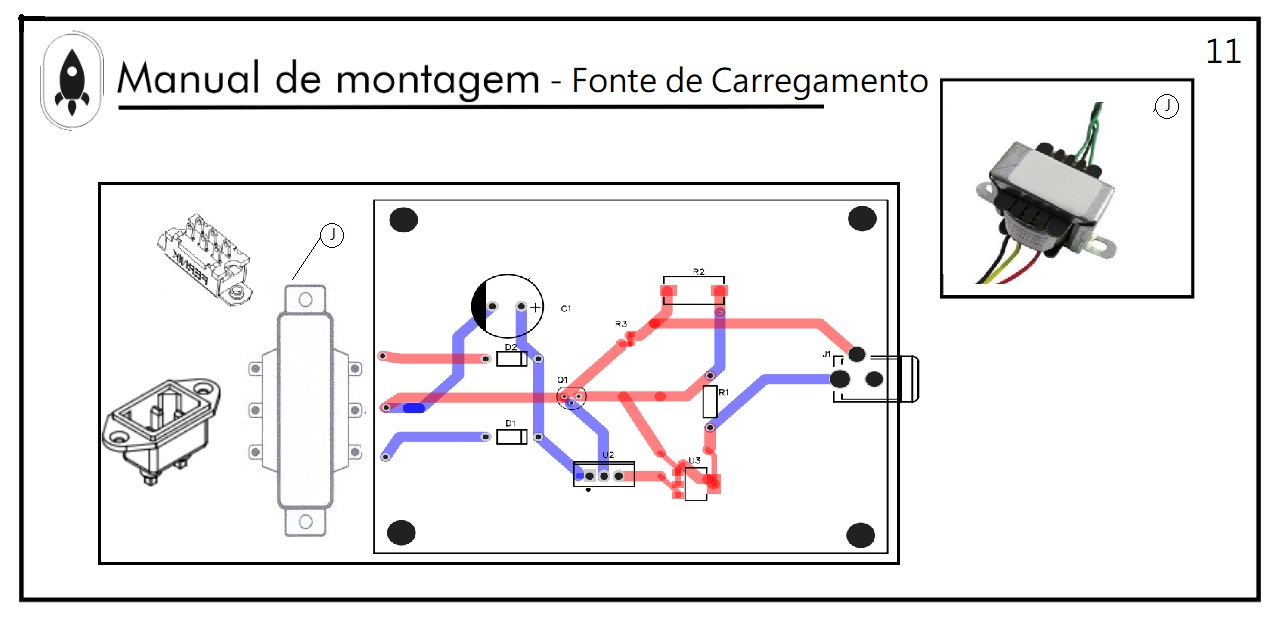
\includegraphics[width=\textwidth]{Figuras/Carregador/carregador_manual_11.jpg}
  \caption{Transformador 110/220V para 30V 1A.} 
 %{ \footnotesize Fonte: Autores} 
  \label{carregador11}
\end{figure}

Em seguida será fixado a chave seletora de tensão HH, figuira \ref{carregador12}, e a tomada de força na estrutura da fonte do carregador, figura \ref{carregador13}. Para fixar use o processo citado anteriormente com uso de parafusos de 40mm e seguindo os passos explicados no item 4.4.

\begin{figure}[H]
  \centering
  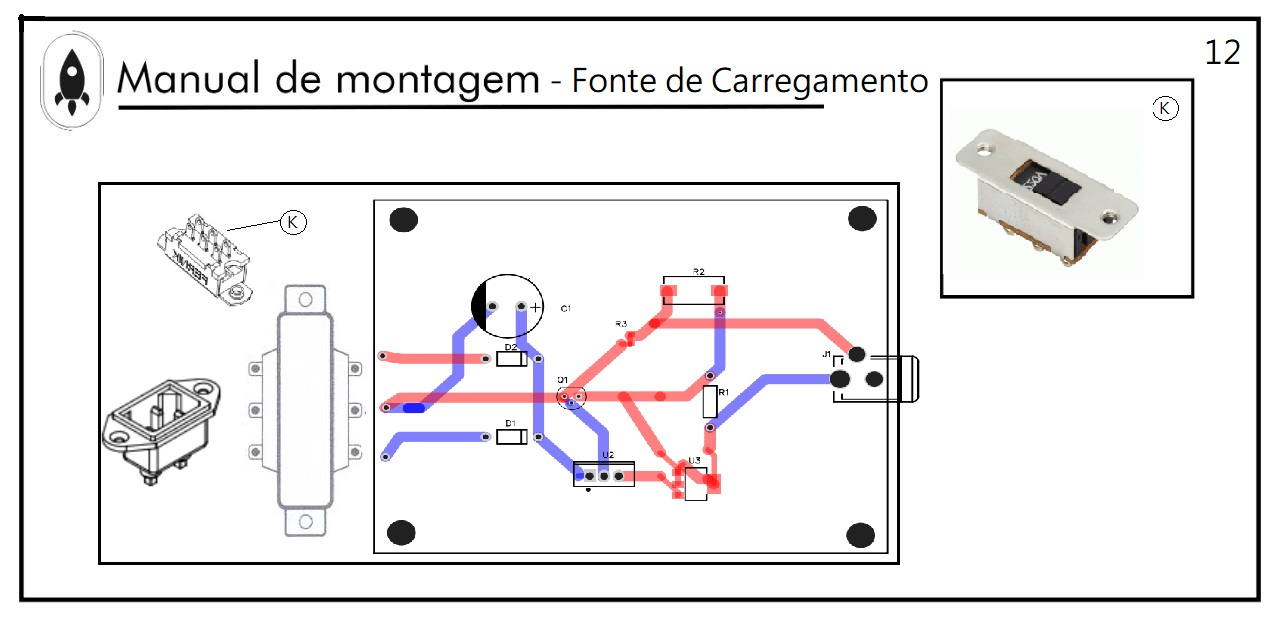
\includegraphics[width=\textwidth]{Figuras/Carregador/carregador_manual_12.jpg}
  \caption{Chave seletora de tensão HH 127/220V.} 
   \label{carregador12}
\end{figure}

\begin{figure}[H]
  \centering
  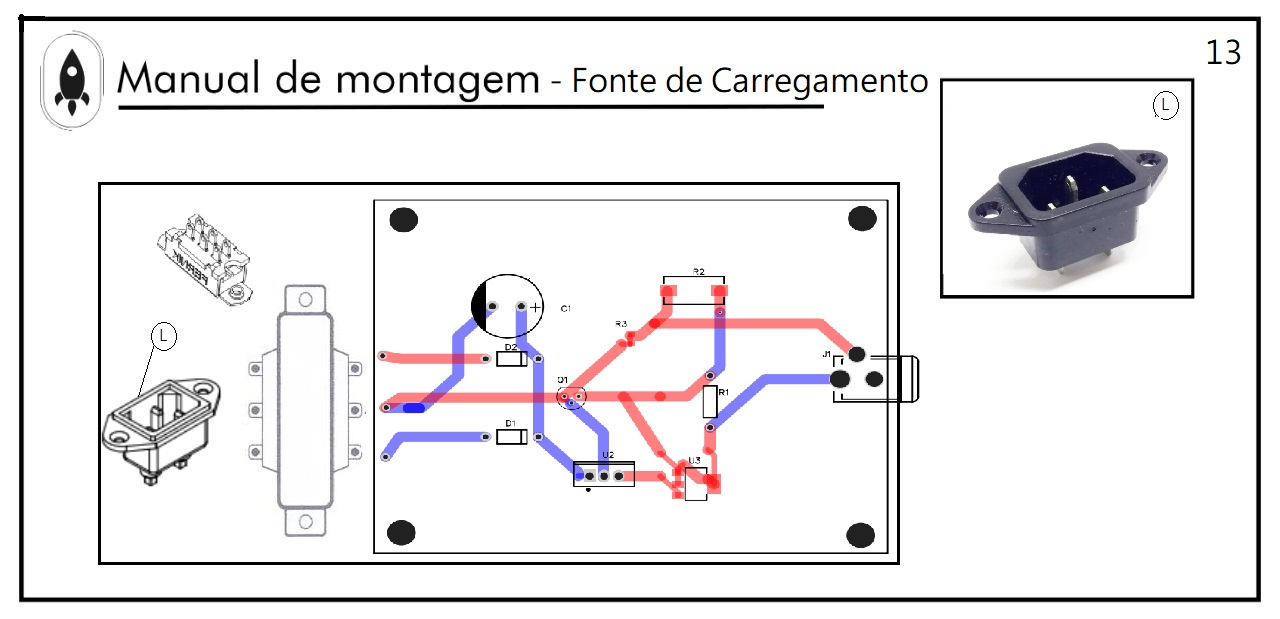
\includegraphics[width=\textwidth]{Figuras/Carregador/carregador_manual_13.jpg}
  \caption{Tomada de força lec 320 C14 - Macho.} 
   \label{carregador13}
\end{figure}

Após a montagem dos dispositivos na estrutura a fonte do carregador estará com os seguintes aspectos, figura \ref{carregador_cad1}, \ref{carregador_cad2} e \ref{carregador_cad3}.

\begin{figure}[H]
  \centering
  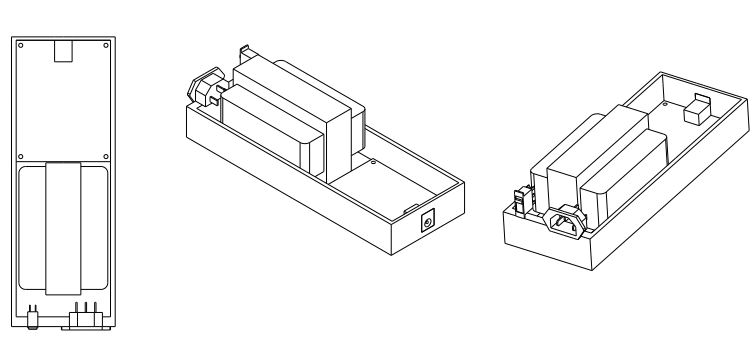
\includegraphics[width=\textwidth]{Figuras/Carregador/Carregador_cad1.JPG}
  \caption{Vistas fonte do carregador.} 
  \label{carregador_cad1}
\end{figure}

\begin{figure}[H]
  \centering
  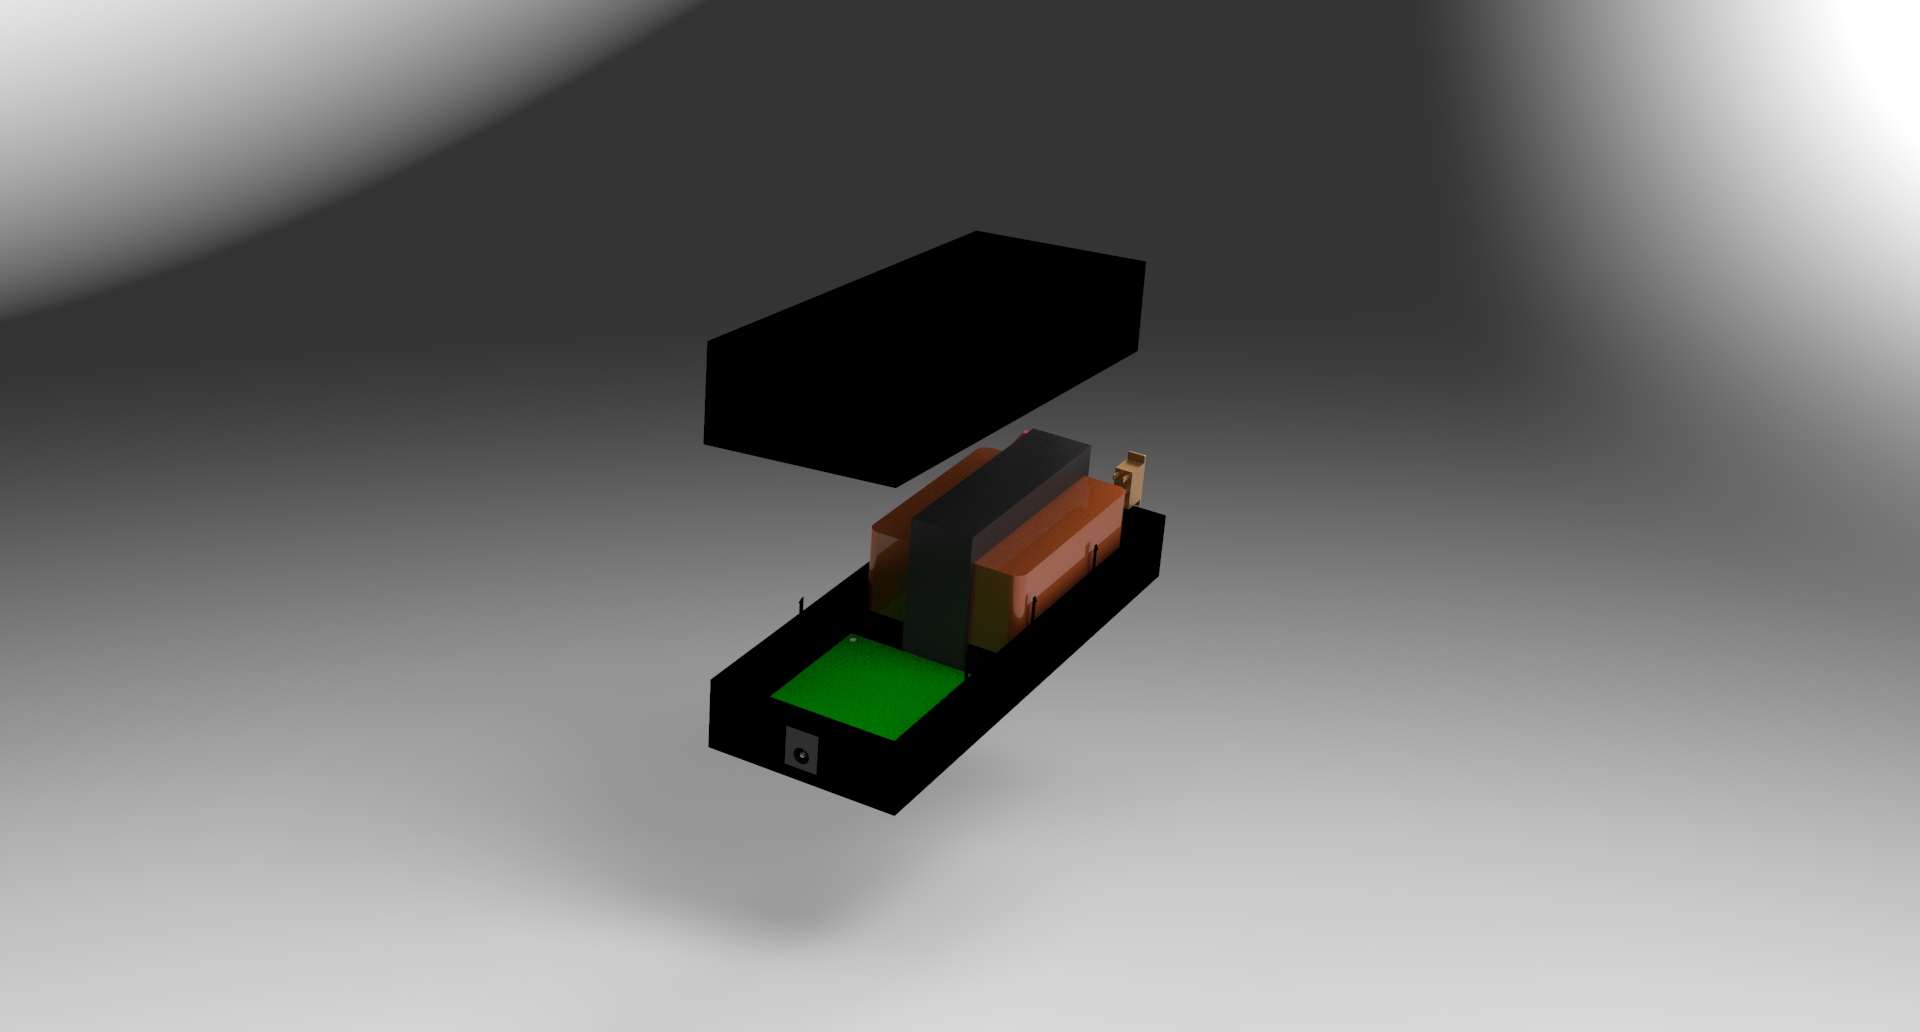
\includegraphics[width=\textwidth]{Figuras/untitled.8.jpg}
  \caption{Fonte do carregador 01.} 
  \label{carregador_cad2}
\end{figure}

\begin{figure}[H]
  \centering
  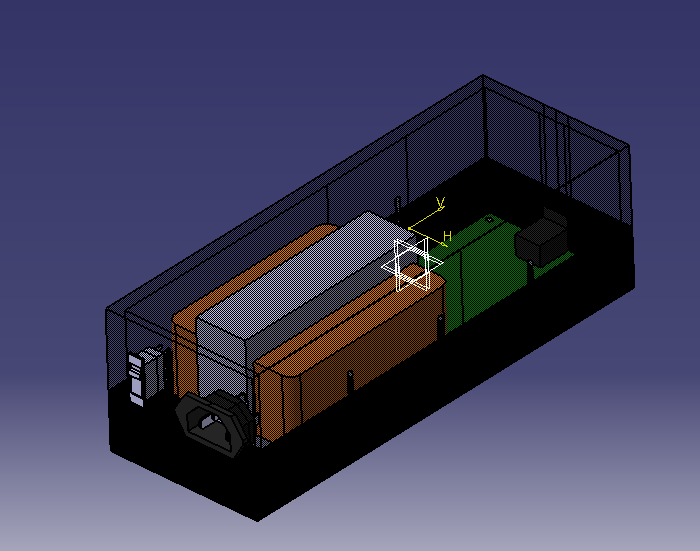
\includegraphics[width=0.8\textwidth]{Figuras/ISOCARREGADOR.PNG}
  \caption{Fonte do carregador 02.} 
  \label{carregador_cad3}
\end{figure}

\newpage

\section{Conexões do Carregador}

Para conectar os dispositivos de acordo com o esquemático apresentado na figura \ref{carregador_conexoes} primeiro é preciso identificar os fios de 220V e 110V no primário do transformador, a maioria dos transformadores já vem com essa informação porém, caso não esteja claro é possível testar com um multímetro seguindo os próximos passos:

\begin{itemize}
    \item Com a ajuda de um multímetro coloque em uma escala baixa de medição de resistência de 2K $\Omega$ 
    \item Com o multímetro meça a resistência entre o fio preto e cada um dos outros dois fios que o acompanha. O fio que com o preto medir a maior valor de resistência esse será o de 220V.
\end{itemize}


\begin{figure}[H]
  \centering
  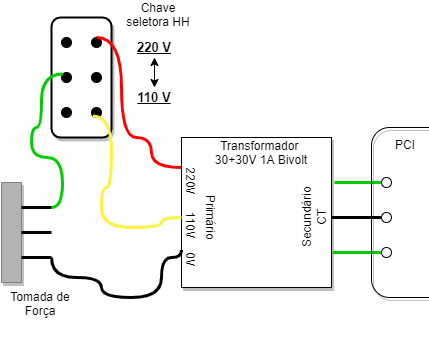
\includegraphics[width=\textwidth]{Figuras/Carregador/conexao_carregador.png}
  \caption{Conexões - Fonte do carregador.} 
 %{ \footnotesize Fonte: Autores} 
  \label{carregador_conexoes}
\end{figure}

Como é apresentado na figura \ref{carregador_conexoes} o fio de 0V é ligado diretamente no neutro da tomada de força, já os fios de 110V e 220V são ligados na chave seletora como mostra o esquemático. Usando um fio de cobre encapado 2,5$mm^2$.

Meça a quantidade de fio necessária para conectar o terminal fase da tomada de força até o terminal no centro da chave seletora HH, corte o tamanho necessário com o uso do alicate, e desencape a ponta do fio com um estilete.

Para conectar os fios nos terminais será usado os terminais Faston Fêmea, esses terminais são usados para evitar a soldagem dos fios e trazer mais praticidade e segurança a conexão. Você irá fixá-los na extremidade dos três fios do primário do transformador e nas duas extremidades do fio verde que conectará a tomada com a chave seletora.

Para fixar os terminais Faston Fêmea basta seguir os passos apresentados na figura \ref{terminal_faston} a seguir.

\begin{figure}[H]
  \centering
  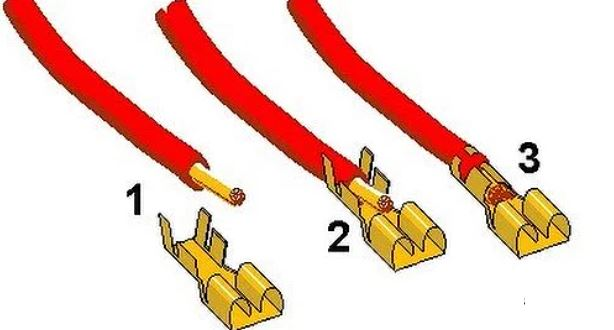
\includegraphics[width=\textwidth]{Figuras/Carregador/terminal_faston.JPG}
  \caption{Conexão Terminal Faston Fêmea.} 
 %{ \footnotesize Fonte: Autores} 
  \label{terminal_faston}
\end{figure}

Após fixar os terminais em cada uma das cinco extremidades basta encaixar os terminais fêmeas nos terminais da tomada de força e da chave seletora como mostrado na figura \ref{carregador_conexoes}.

Para os fios do secundário do transformador basta soldá-los nos terminais da PCI do carregador, atente-se para que o fio de center tape do transformador seja soldado no terminal central da PCI como mostra a figura \ref{carregador_conexoes}.

Depois de feito todas as conexões da fonte feche a fonte com a tampa da sua estrutura fazendo com que os pinos lateria da estrutura se encaixe perfeitamente. 

\section{Cabos do Carregador}

O carregador de baterias terá dois cabos que será conectado em cada uma das suas duas extremidades.

\begin{itemize}
    \item Cabo para a conexão com a rede elétrica : Cabo de força Plug Macho 3 Pinos Redondo de 4,00mm, Cabo com 3 fios internos de 0,75$mm^2$ (2,5m) e com um Plug IEC C13 
    \item Cabo para a conexão com a maleta ou base de lançamento: Cabo PP 2X2,5$mm^2$ Preto com conectores Jack J4 nas duas extremidades do cabo.
\end{itemize}

Para fazer o cabo que conecta na maleta ou base é preciso, primeiro, desencapar cerca de 1cm da ponta dos dois fios (positivo e negativo) do Cabo PP nas duas extremidades do cabo, depois disso, desenroscar os Plugs Jack macho e com a solda fixar em cada lado o fio positivo (cor azul) e negativo (cor preta) no plug como é apresentado na figura \ref{conexao_jack}.


\begin{figure}[H]
  \centering
  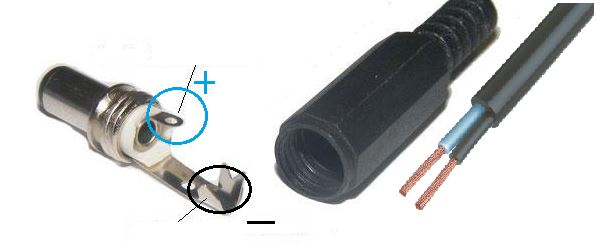
\includegraphics[width=\textwidth]{Figuras/Carregador/conexao_jack.JPG}
  \caption{Conexão do cabo no plug Jack Macho..} 
 %{ \footnotesize Fonte: Autores} 
  \label{conexao_jack}
\end{figure}

Após soldar os fios, enrosque novamente o os Plugs Jack macho e certifique-se que estão bem presos. 